\documentclass[11pt,dvipsnames]{scrreprt}

\usepackage[utf8]{inputenc}
\usepackage[ngerman]{babel}
\usepackage{fullpage} 			% kleinere Ränder

\usepackage{comment} 			% für größere comments: \begin{comment} ... \end{comment}
\usepackage{lscape} 			%für landscape-format

% *** für eingefügte (pdf-)Grafiken
\usepackage[pdftex]{graphicx}
\usepackage{epstopdf}
\usepackage{epsfig}
%\pdfminorversion=6
% ***

\usepackage{float} 
\usepackage{enumerate} 			%für geschachtelte Aufzählungen

\linespread{1.25}
\usepackage{amsmath} 			%Matheformeln usw.
\usepackage{amssymb} 			%mathfrak

\usepackage[bookmarks=true]{hyperref} 	% hyperrefs aktivieren
\setcounter{secnumdepth}{3} 		%Numerierung bis Tiefe 3, also ab \paragraph ohne
\setcounter{tocdepth}{1}

\usepackage{multirow}	 		%für Multirow Tabellen
\usepackage{forloop,supertabular}	% mehrseitige Tabellen
\usepackage{tabularx}
\usepackage{pbox}

\usepackage{chngcntr}  			%Nummerierung neu beginnen
%\counterwithout{figure}{chapter}

%Farben
\usepackage{xcolor}
\usepackage{tikz}
\usetikzlibrary{shapes,snakes}

\usepackage{multicol}
\usepackage{dirtree}
\usepackage{minitoc}



%*** title usw.
\title{Dokumentation \\
    zur Studienarbeit im Fach\\
Praktikum Softwareengineering\\
\vspace{1cm}
- Entwicklung einer Lernsoftware -\\
"myMemo"\\
\vspace{5cm}
}
\author{ von Susanne Kießling\\
\vspace{2cm}
    Dozent: Prof. Dr. Martin Thost}
\date{\today}


\begin{document}
\maketitle
\tableofcontents

\clearpage

\chapter{Anforderungen des Kunden}
Die Diakonie Hochfranken möchte das Angebot an Lernsoftware in ihren Kindergärten und Kindertagesstätten erweitern. Es soll eine Lernsoftware entwickelt werden, die Gedächtnistraining und die Erweiterung des Wortschatzes spielerisch umsetzt.

\section{Systemvoraussetzungen}
Aktuell verfügt der Kunde über Einzelplatz-PC's, die in den Jahren 2005 bis 2010 angeschafft wurden. Als Betriebssystem kommt Linux und Windows zum Einsatz.

\section{Zielgruppe}
Die Besucher der Einrichtung im Alter von fünf bis zehn Jahren bilden die Zielgruppe der Software. 


\clearpage
\chapter{Lastenheft}

\section{Zielbestimmung} %welche Ziele sollen mit dem Software-Produkt erreicht werden.
Mit der Lernsoftware wird die Möglichkeit geschaffen, das pädagogisch wertvolle Prinzip des klassischen Memory-Spiel auf eine digitale Plattform zu übertragen. Zusätzlich zum Gedächtnistraining trägt die Vokabelfunktion zur Erweiterung des Wortschatzes bei. Die Führung einer Highscore ermöglicht den Vergleich der erreichten Punkte und steigert die Motivation der Benutzer, eine bessere Platzierung zu erreichen. Das erhöht wiederum den Lerneffekt. Neben dem Spielen an sich wird der Umgang mit dem Computer spielerisch erlernt. Vor Spielbeginn sind Attribute festzulegen und Meldungen der Software zu beachten. Das schult zusätzlich die Logik. Der 2-Player-Modus unterstützt außerdem die Kommunikation mit anderen Spielern.


\section{Produkteinsatz} %Anwendungsbereiche und Stakeholders werden genannt
Die Lernsoftware kommt in den Kindertagesstätten der Diakonie Hochfranken zum Einsatz. Anwender der Software sind Besucher der Kindertagesstätte im Alter von fünf bis zehn Jahren.

\section{Produktfunktionen} %Hauptfunktionen werden beschrieben, Stakeholdergruppen
%zugeordnet und in 10er-Schritten durchnummeriert (LF nn).

\noindent Priorität 1:\\
\noindent$\backslash$LF10$\backslash$ \hspace{15 mm}Spieler neu erstellen \\
\noindent$\backslash$LF11$\backslash$ \hspace{15 mm}Spieler laden\\ % prüfen, ob Spieler bereits vorhanden
\noindent$\backslash$LF12$\backslash$ \hspace{15 mm}Spielerdaten ändern\\  % löschen, ändern usw.
%\vspace{10 mm}
\noindent$\backslash$LF20$\backslash$ \hspace{15 mm}Anzahl der Spieler wählen\\
\noindent$\backslash$LF30$\backslash$ \hspace{15 mm}Thema wählen\\
\noindent$\backslash$LF40$\backslash$ \hspace{15 mm}Spielfeldgröße wählen\\
\noindent$\backslash$LF50$\backslash$ \hspace{15 mm}Spiel starten\\

\noindent $\backslash$LF60$\backslash$ \hspace{15 mm}Highscore anzeigen\\

\noindent Priorität 2:\\
\noindent$\backslash$LF70$\backslash$ \hspace{15 mm}Urkunde drucken\\
\noindent$\backslash$LF80$\backslash$ \hspace{15 mm}Vokabeltraining\\
\noindent$\backslash$LF90$\backslash$ \hspace{15 mm}Audiodaten abspielen \\ 


\section{Produktdaten} %permanent gespeicherte Hauptdaten werden festgelegt und in
%10er-Schritten durchnummeriert (LD nn).
$\backslash$LD10$\backslash$ \hspace{15 mm}Spielerdaten \\ \\
\noindent $\backslash$LD20$\backslash$ \hspace{15 mm}Highscoredaten \\ \\

\section{Produktleistungen} % besondere Anforderungen an Hauptfunktionen oder Haupt-
%daten (Ausführungszeit, Datenumfang, ... ) werden aufgezählt (LL nn).

\section{Qualitätsanforderungen} % allgemeine Eigenschaften wie gute Zuverlässigkeit,
%hervorragende Benutzbarkeit, normale Effizienz, ... werden festgelegt.
Funktionalität:	\hspace{15 mm}		gut\\
Zuverlässigkeit:\hspace{15 mm}		sehr gut\\
Benutzbarkeit:	\hspace{15 mm}		gut\\
Effizienz:	\hspace{15 mm}		normal\\
Änderbarkeit:	\hspace{15 mm}		normal\\
Portierbarkeit:	\hspace{15 mm}		sehr gut\\
Spassfaktor:	\hspace{15 mm}		sehr gut\\
\section{Ergänzungen} % alles was nicht in obiges Schema passt und trotzdem wichtig ist.
Die Umsetzung der Software erfolgt in der Programmiersprache Java. Da der Kunde Linux und Windows als Betriebssystem einsetzt stellt dies die notwendige Portierbarkeit sicher.



\clearpage
\chapter{Aufwandskalkulation}
Die Aufwandskalkulation für die Planung, Analyse, Design, Konstruktion, Test und Einführung der Software wird anhand des Funktionspunktverfahren durchgeführt.

\clearpage
\section{Function Point Methode}
\begin{figure}[!h]
	\centering
    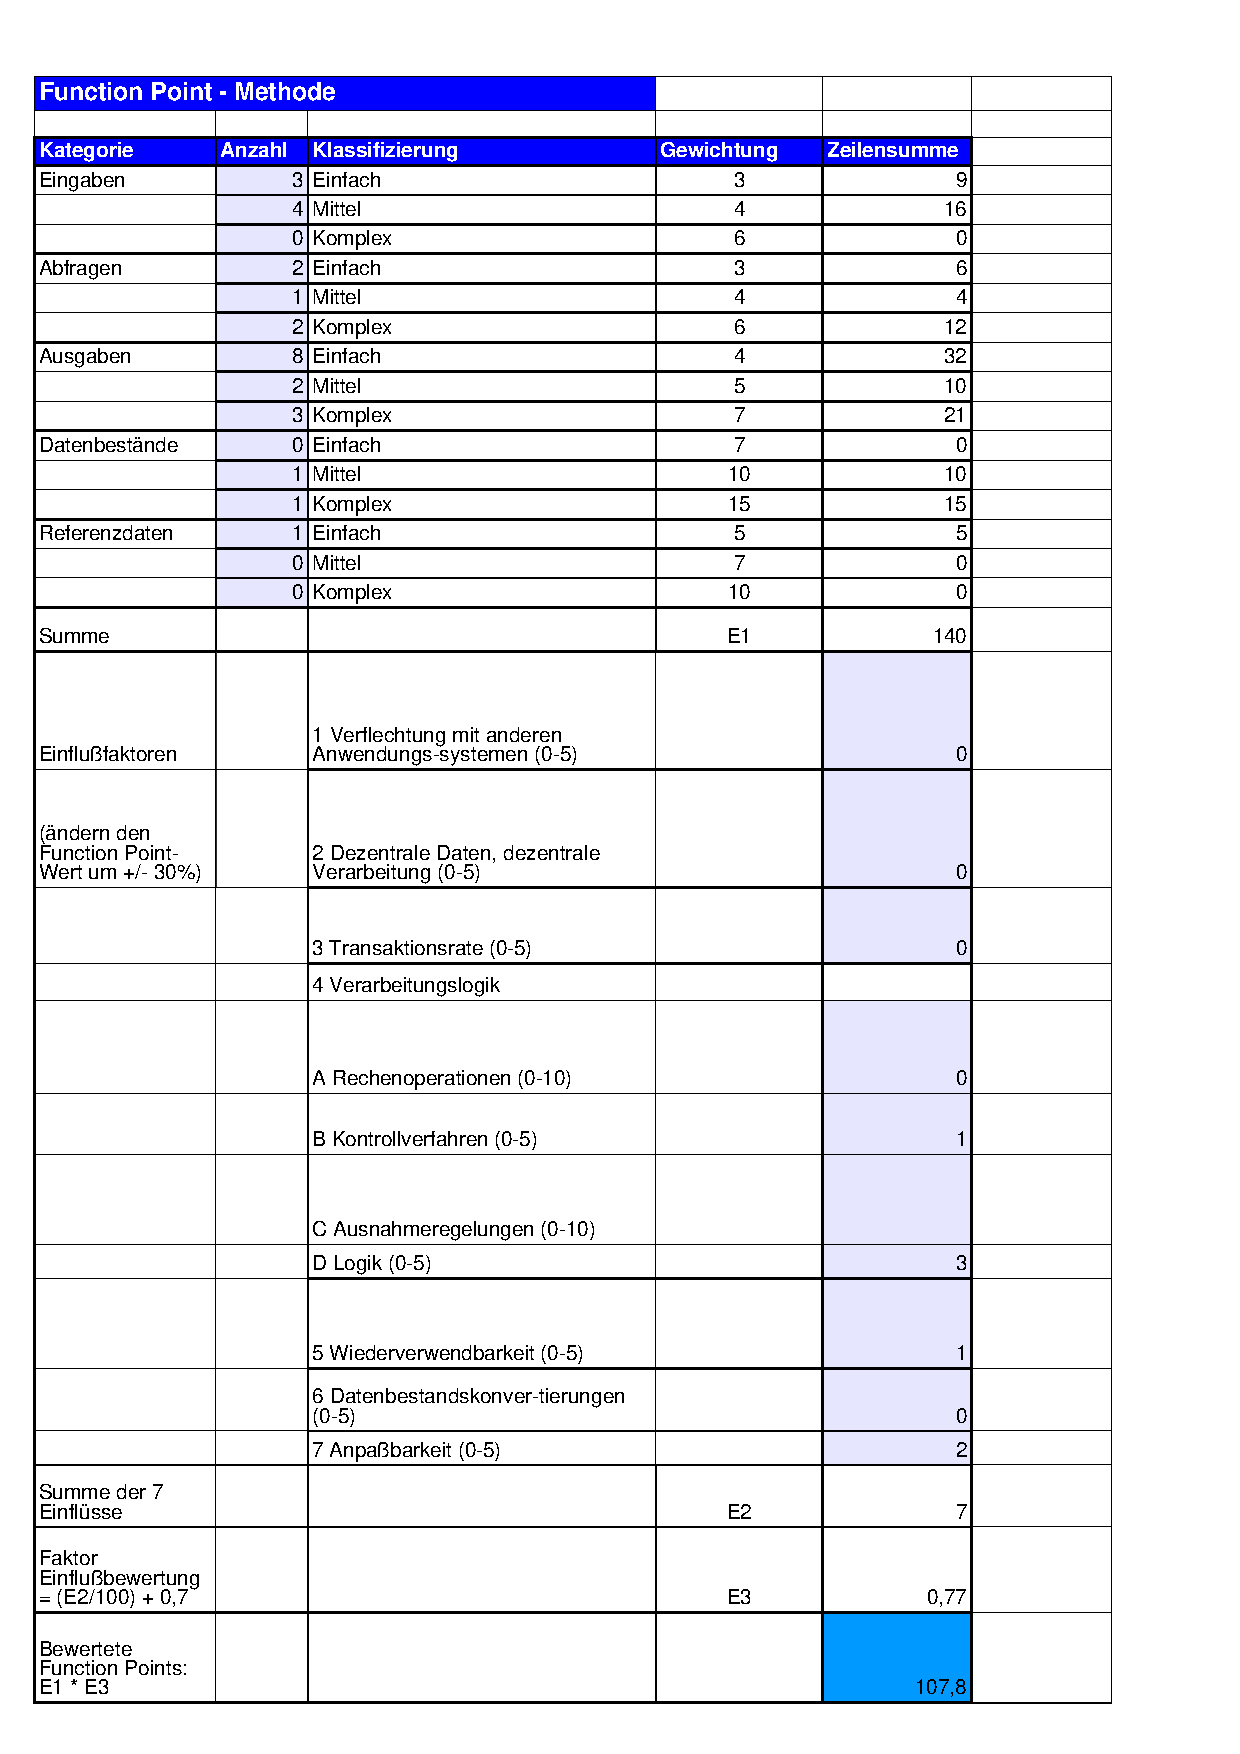
\includegraphics[width=15cm]{./FunctionPoint_filled.pdf}
	\label{layout_gesamt}
\end{figure}


\clearpage

\chapter{Projektplan}
Das Projekt wird von Kalenderwoche 12 - 2013 bis Kalenderwoche 29 - 2013 durchgeführt. Der Projektplan gibt Anhaltspunkte, welche Projektphasen wann abgeschlossen sein müssen.\\ \\

\begin{figure}[!h]
	\centering
    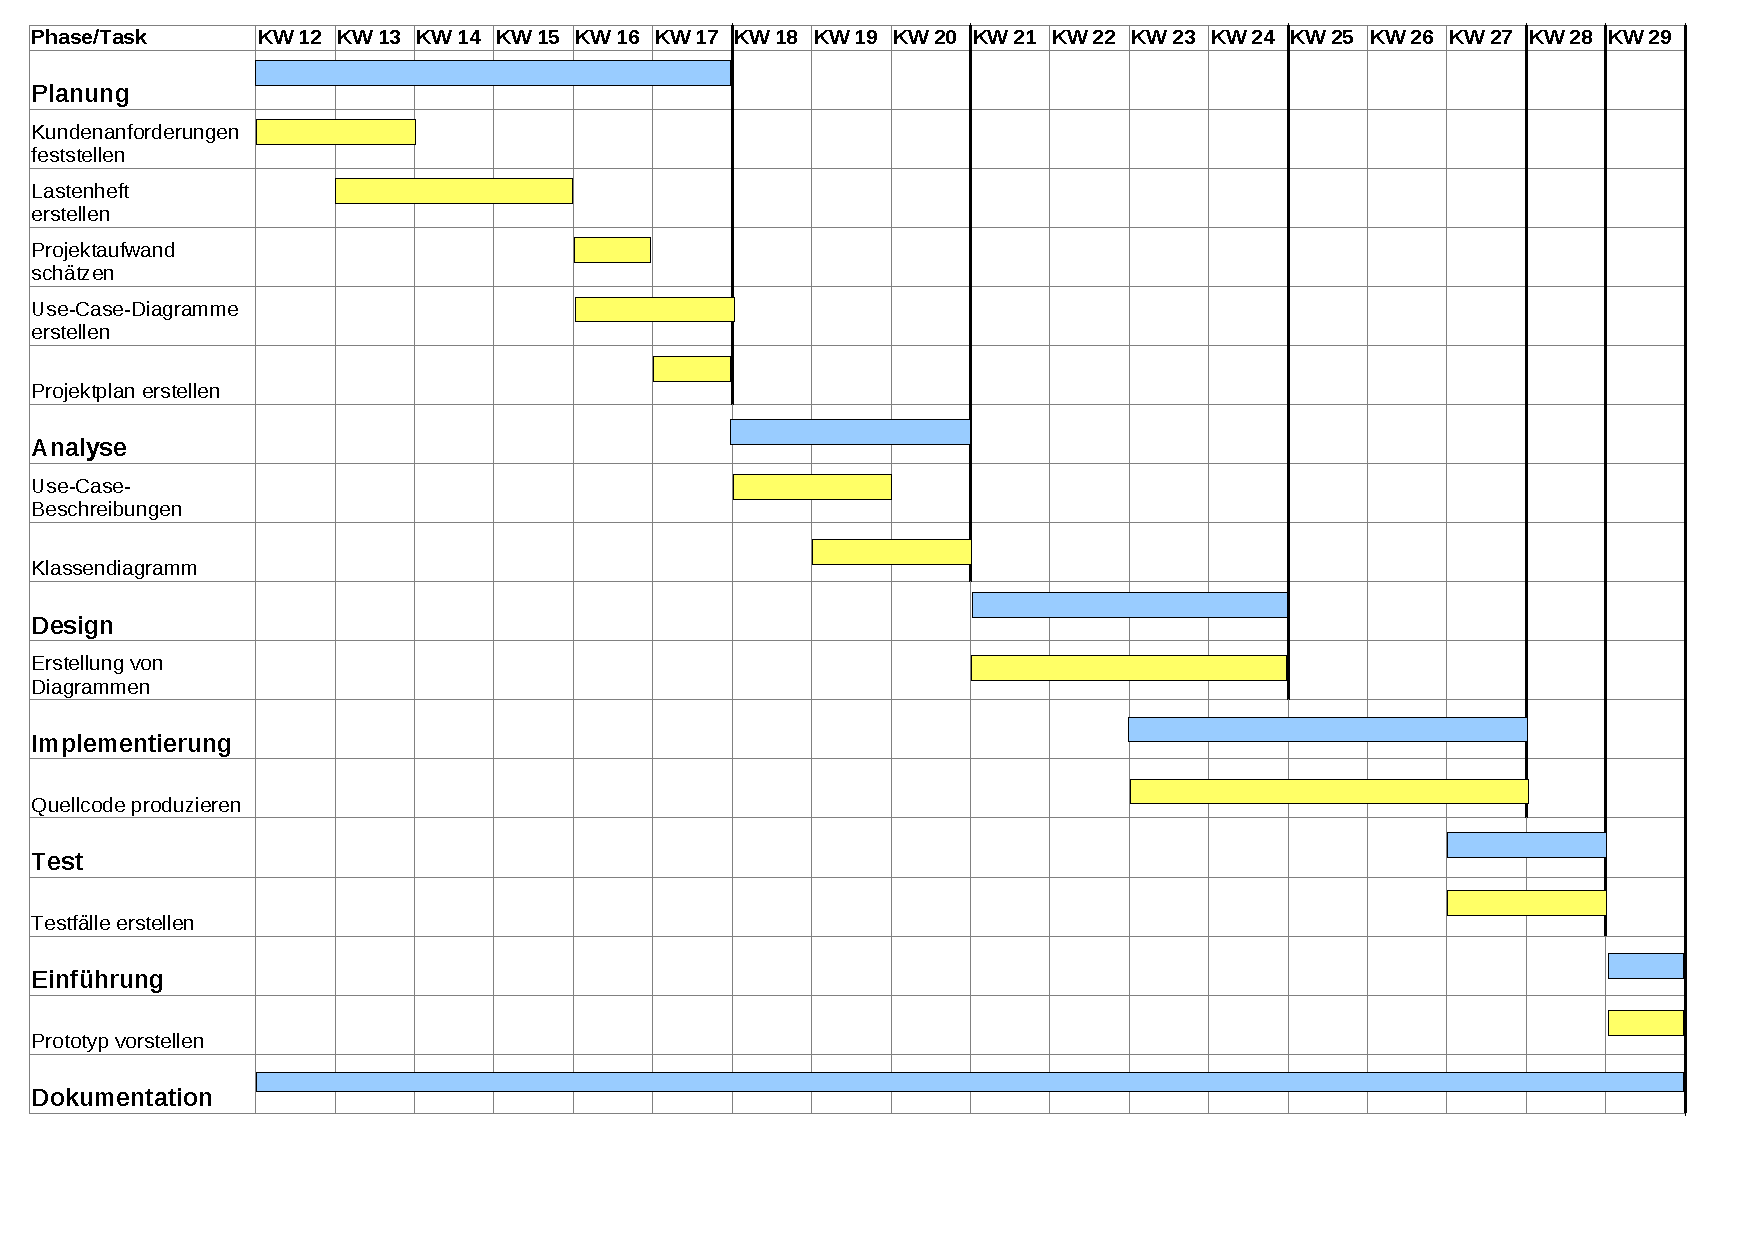
\includegraphics[width=\textwidth]{./projektplan.pdf}
	\label{layout_gesamt}
\end{figure}



\clearpage

\chapter{Use Case Diagramme}


\section{}


\section{}



\clearpage

\chapter{Use Case Beschreibungen}


\section{Spieler erstellen}
\begin{tabular}{|l|l|l|l|l|l|l|}
\hline
\textbf{Use Case:} & \multicolumn{ 6}{l|}{Spieler erstellen} \\ \hline
\textbf{Actors:} & \multicolumn{ 6}{l|}{Benutzer} \\ \hline
\textbf{Purpose:} & \multicolumn{ 6}{l|}{Benutzer erstellt durch Eingabe seines Namens einen Spieler} \\ \hline
\textbf{Entry Cond:} & \multicolumn{ 6}{c|}{} \\ \hline
\textbf{Overview:} & \multicolumn{ 6}{l|}{Für den Benutzer ist noch kein Spieler erstellt. Der Benutzer trägt seinen Namen ein 
und erstellt somit einen neuen Spieler.} \\ \hline
\textbf{Exit Cond:} & \multicolumn{ 6}{l|}{} \\ \hline
\textbf{Includes:} & \multicolumn{ 6}{l|}{} \\ \hline
\textbf{Special Req:} & \multicolumn{ 6}{l|}{} \\ \hline
\textbf{Category:} & \multicolumn{ 6}{l|}{} \\ \hline
\textbf{Cross Ref:} & \multicolumn{ 6}{l|}{auf /LF10/ aus Lastenheft} \\ \hline
\textbf{Ablauf:} & \multicolumn{ 3}{l|}{Actor Action:} & \multicolumn{ 3}{l|}{System Response:} \\ \hline
\multicolumn{ 1}{|c|}{} & \multicolumn{ 3}{l|}{1. Spieler erstellen wählen} & \multicolumn{ 3}{l|}{} \\ \cline{ 2- 7}
\multicolumn{ 1}{|l|}{} & \multicolumn{ 3}{l|}{2. Spielernamen eintragen} & \multicolumn{ 3}{l|}{} \\ \cline{ 2- 7}
\multicolumn{ 1}{|l|}{} & \multicolumn{ 3}{l|}{} & \multicolumn{ 3}{l|}{} \\ \cline{ 2- 7}
\multicolumn{ 1}{|l|}{} & \multicolumn{ 3}{l|}{} & \multicolumn{ 3}{l|}{} \\ \cline{ 2- 7}
\multicolumn{ 1}{|l|}{} & \multicolumn{ 3}{l|}{} & \multicolumn{ 3}{l|}{} \\ \cline{ 2- 7}
\multicolumn{ 1}{|l|}{} & \multicolumn{ 3}{l|}{} & \multicolumn{ 3}{l|}{} \\ \hline
\end{tabular}


\clearpage
\section{Spieler laden}

\clearpage
\section{Spielmodus wählen}

\clearpage
\section{Thema wählen} 

\clearpage
\section{Spielfeldgröße wählen}

\clearpage
\section{Spiel starten}

\clearpage
\section{Highscore anzeigen}

\clearpage

\chapter{Klassendiagramm}
Das Klassendiagramm enthält die folgenden Klassen:\\

\noindent \textbf{Main: } Start des Programms, Daten werden von Festplatte geladen \\ \\
\textbf{Menue: } Hauptmenue wird geladen, Eingabedaten des Benutzers entgegengenommen, die Klassen InputData, GameLayout, GameField und GameController werden erstellt \\ \\
\textbf{Card: } Stellt die Funktionen der Memorykarte zur Verfügung, informiert GameController bei Auswahl einer Karte \\ \\
\textbf{GameField: } erstellt das Spielfeld, mischt Karten\\ \\
\textbf{GameLayout: } liefert das Layout für das Spielfeld, wird von Player und GameController über Änderungen benachrichtigt, um geänderte Daten (z.B. Punkte) auf der GUI anzuzeigen\\ \\
\textbf{GridBagLayoutModel: }Hilfsklasse für GameLayout\\ \\
\textbf{InputData: } Datenspeicher für Spieler und Spielmodus\\ \\
\textbf{Player: } repräsentiert den Spieler und seine Daten, enthält Funktion um Punkte hinzuzufügen\\ \\
\textbf{Playerpool: } Verwaltet alle gespeicherten Spieler\\ \\
\textbf{GameController: } Steuert den Spielablauf\\ \\
\textbf{SaveObject: } Nimmt Playerpool und Highscore auf um sie gekapselt zu speichern\\ \\
\textbf{Highscore: } Verwaltet HighscoreData-Objekte, stellt sortierte Liste der 10 Besten Spieler bereit\\ \\
\textbf{HighscoreData: } Enthält Spieler und die erreichten Punkte pro gespieltem Spiel \\ \\
\textbf{HddSave: } Stellt Funktionen zum Speichern und Laden des SaveObjects bereit\\ \\
\textbf{WindowModel: } Vorlage für ein modifiziertes JFrame, wird von der Klasse Menue und GameLayout genutzt \\ \\

\textbf{Bemerkung: }Für die Klassen Menue,GameLayout und GameController sind im Klassendiagramm aufgrund der Übersichtlichkeit und Platzmangels nicht alle Membervariablen abgebildet. Deshalb sind diese zusätzlich mit vollständigen Membervariablen nach dem Klassendiagramm aufgeführt.
    
 
\begin{figure}[!h]
	\centering
    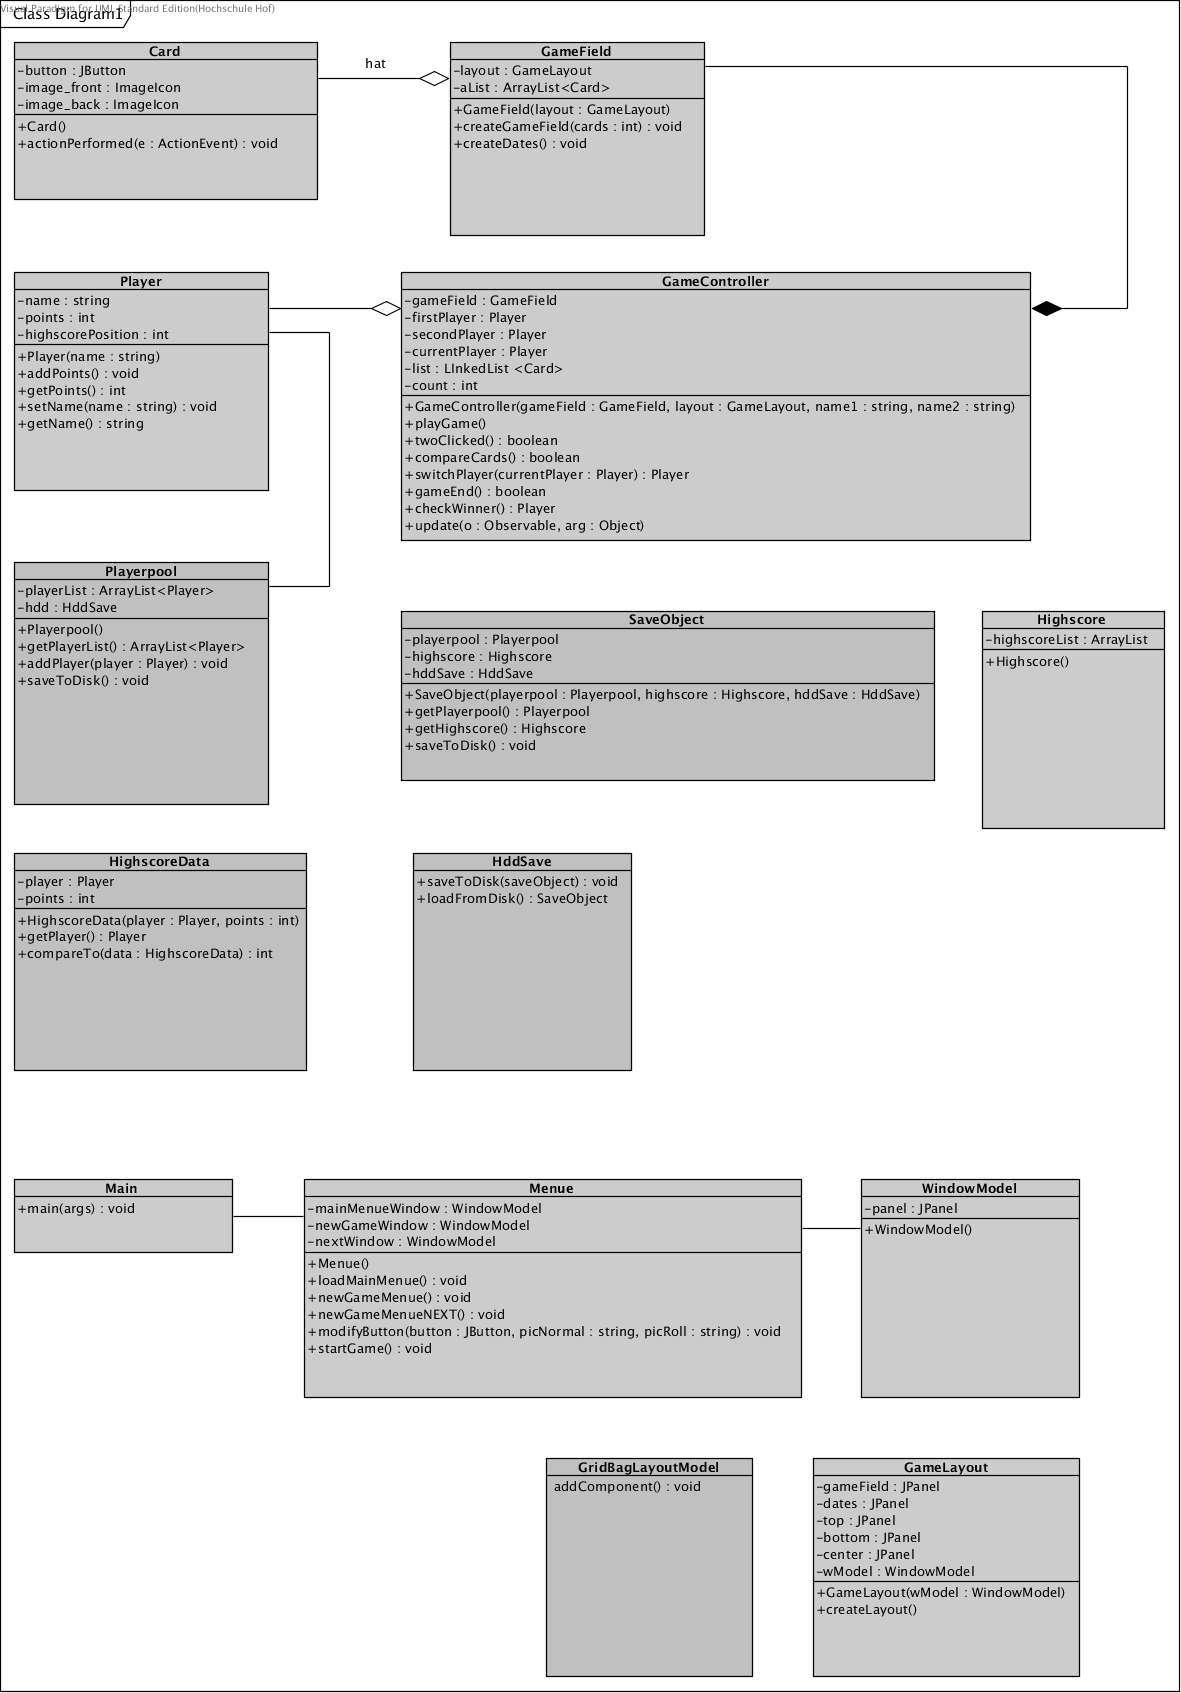
\includegraphics[width=\textwidth]{./Klassendiagramm.png}
	\label{layout_gesamt}
\end{figure}

\begin{figure}[!h]
	\centering
    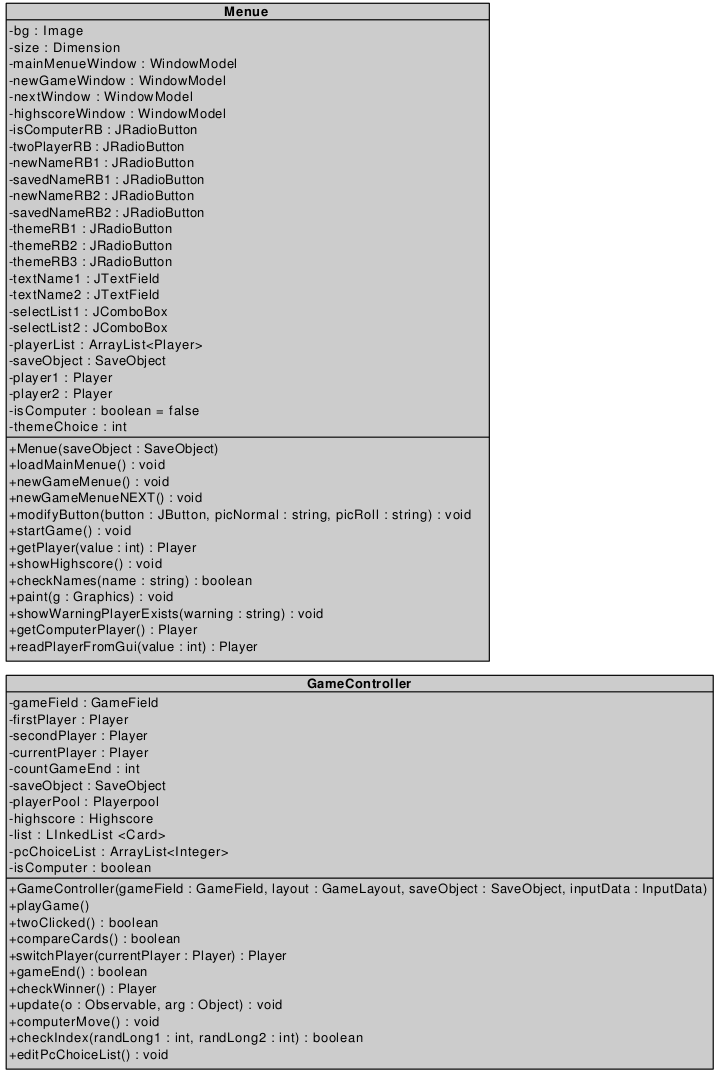
\includegraphics[width=\textwidth]{./Klassendiagramm2.png}
	\label{layout_gesamt}
\end{figure}

\begin{figure}[!h]
	\centering
    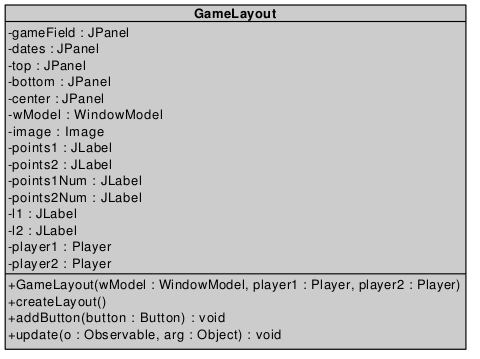
\includegraphics[width=\textwidth]{./Klassendiagramm3.png}
	\label{layout_gesamt}
\end{figure}







\clearpage

\chapter{Sequenzdiagramme}
Sequenzdiagramme modellieren typische Szenarien eines Systems. Es wird die Kommunikation zwischen
Einheiten dargestellt.\\ \\
Folgende Use Cases wurden ausgewählt, um deren Kommunikation anhand von Sequenzdiagrammen darzustellen:\\
\begin{itemize}
  \item Spieler erstellen
  \item Spieler laden
  \item Spiel starten
\end{itemize}

\clearpage
\section{SD Spieler erstellen}
\begin{figure}[h!]
	\centering
    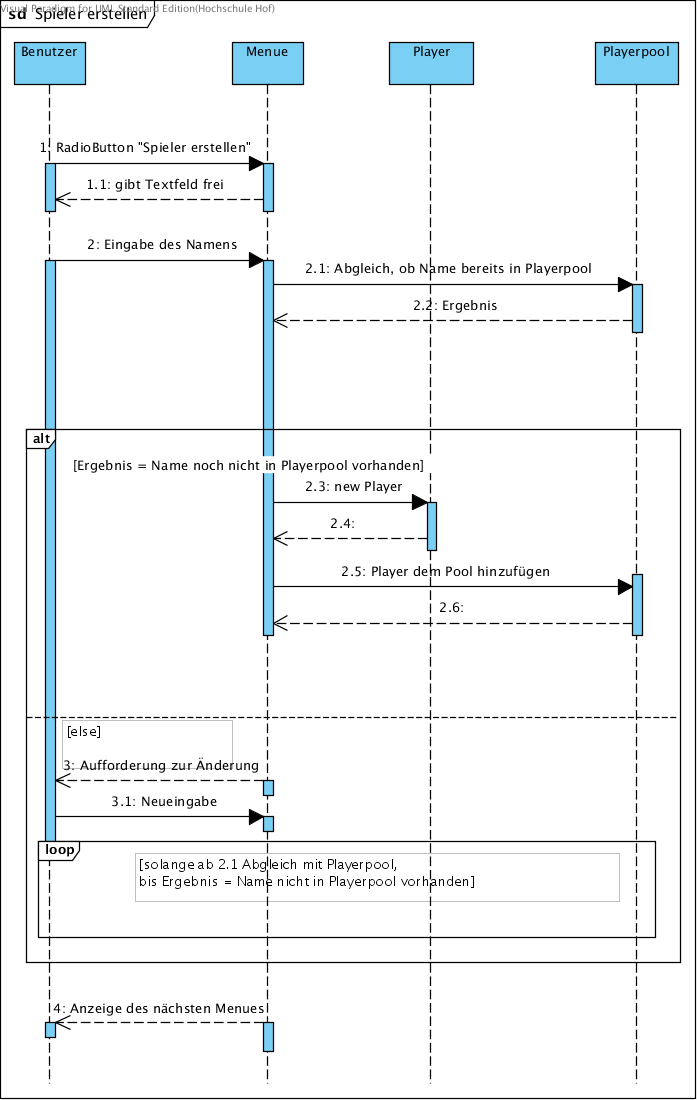
\includegraphics[width=13cm]{./SD_Spieler_erstellen.png}
	\label{layout_gesamt}
\end{figure}
\subsection{Beschreibung}
Der Benutzer wählt den Radio Button ,,Spieler erstellen''. Das Menue gibt das zugehörige Textfeld zur Eingabe des Namens frei. Nach Eingabe des Namens erfolgt ein Abgleich mit dem Playerpool, ob bereits ein Spieler unter diesem Namen gespeichert ist. Das Ergebnis wird zurück zur Klasse Menue geliefert. Ergibt die Prüfung, dass der Name noch nicht vorhanden ist, wir ein neues Objekt vom Typ Player erzeugt und anschließend dem Playerpool hinzugefügt. Ist der eingegebene Name bereits im Playerpool vorhanden, wird der Benutzer aufgefordert, einen anderen Namen einzugeben. Die Prüfung und Neueingabe erfolgt so lange, bis die Prüfung das Ergebnis = noch nicht im Playerpool vorhanden, liefert. Abschließend wird die nächste Menueseite angezeigt.

\clearpage
\section{SD Spieler laden}
\begin{figure}[h!]
	\centering
    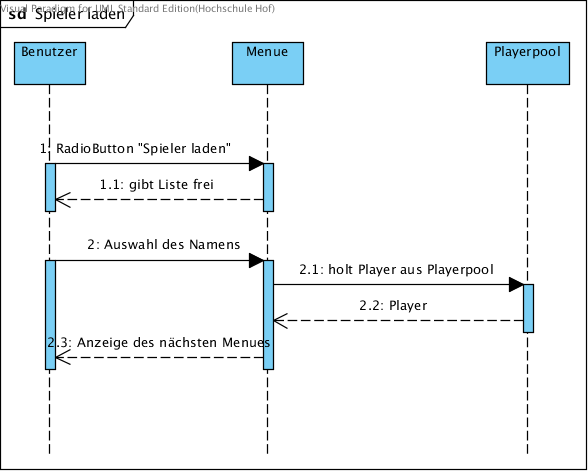
\includegraphics[width=\textwidth]{./SD_Spieler_laden.png}
	\label{layout_gesamt}
\end{figure}
\subsection{Beschreibung}
Der Benutzer klickt den Radio Button ,,Spieler laden'' an. Daraufhin wird durch die Klasse Menue eine Liste der gespeicherten Spieler als Dropdown-Liste freigegeben. Daraus kann der Benutzer den gewünschten Namen wählen. Das Menue nimmt die Auswahl entgegen und holt sich den entsprechenden Player aus dem Playerpool. Anschließend wird die nächste Maske angezeigt.

\clearpage
\section{SD Spiel starten}
\begin{figure}[h!]
	\centering
    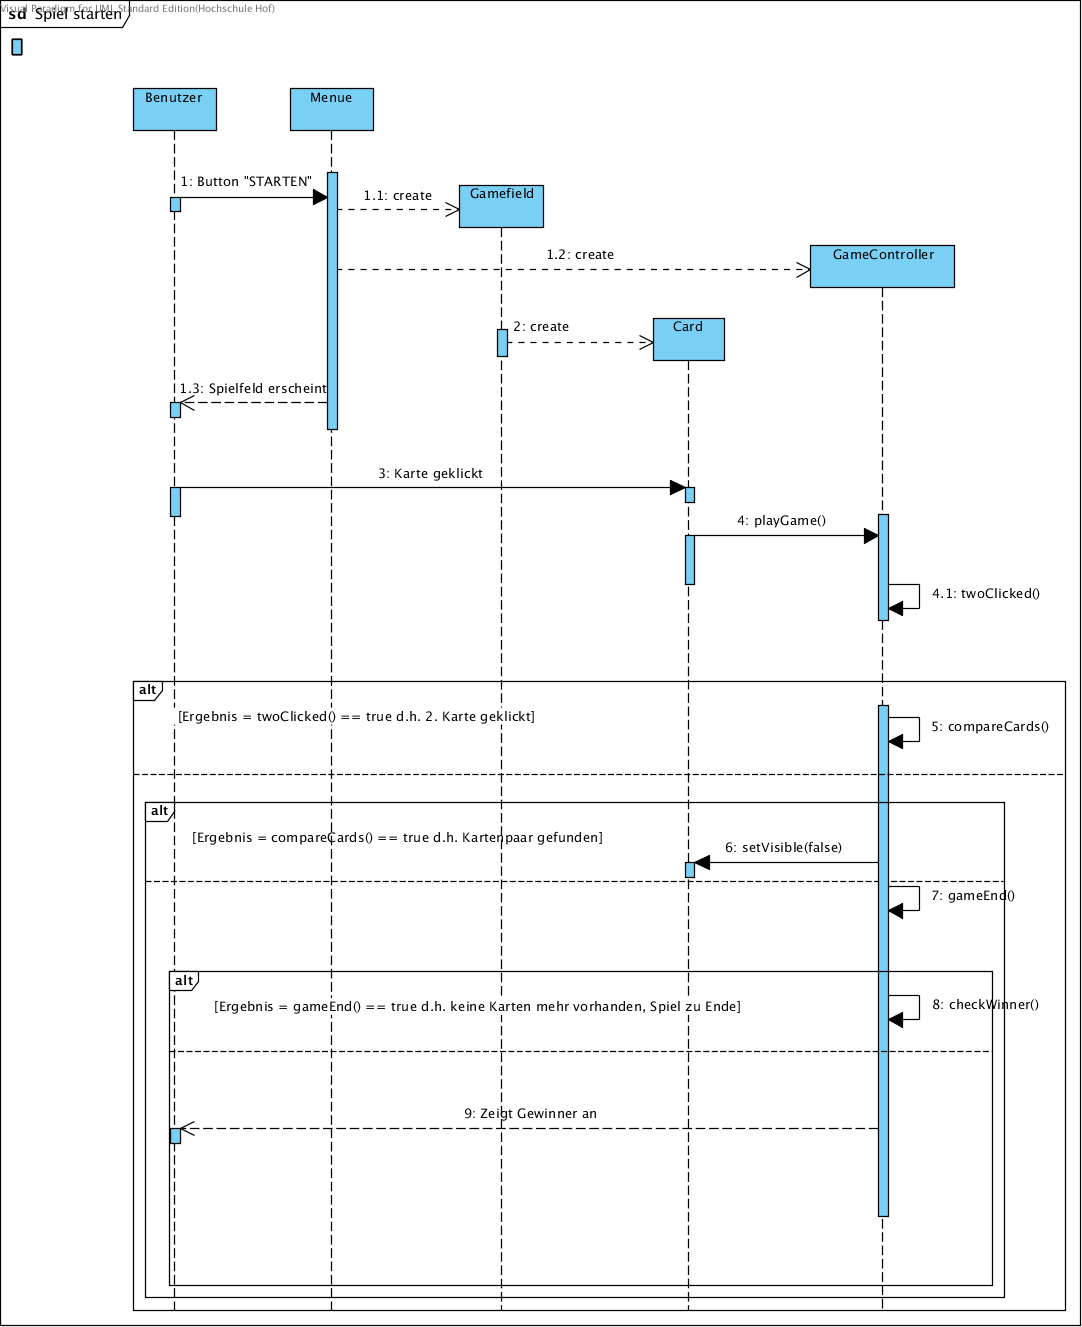
\includegraphics[width=15cm]{./SD_Spiel_starten.png}
	\label{layout_gesamt}
\end{figure}
\subsection{Beschreibung}
Der Benutzer drückt den Button ,,STARTEN``. Daraufhin werden von der Klasse Menue die Klassen GameField und GameController erstellt. Von GameField wird die Klasse Card erstellt. Hier werden die von der Klasse Menue übergebenen Parameter zum Erstellen des Spielfelds verarbeitet und die Karten gemischt. Anschließend wird dem Benutzer das Spielfeld angezeigt. Vom Benutzer wird eine Karte angeklickt. Dies wird in der Klasse Card aufgenommen und durch den Aufruf der Methode playGame() an den GameController weitergegeben. Der GameController ruft die Methode twoClicked() auf. Ist das Ergebnis true, wird die Methode compareCards() aufgerufen. Hat die Prüfung ergeben, dass die Karten übereinstimmen, werden die jeweiligen Karten mit der Methode setVisible(false) unsichtbar gemacht. Anschließend wird geprüft, ob das Spiel zu Ende ist. Trifft dies zu, wird die Methode checkWinner() aufgerufen und der hiermit ermittelte Gewinner dem Benutzer angezeigt. 






\clearpage

\chapter{Weitere Diagramme}

\section{Zustandsdiagramm - Memorykarte}

\begin{figure}[!h]
	\centering
    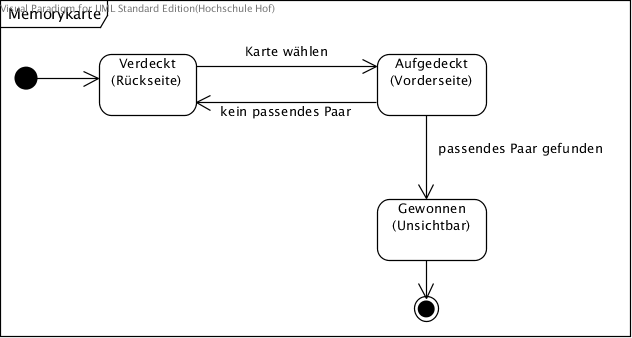
\includegraphics[width=\textwidth]{./ZD_Memorykarte.png}
	\label{layout_gesamt}
\end{figure}
\subsection{Beschreibung}
Die Karte kann die drei Zustände Verdeckt, Aufgedeckt und Gewonnen annehmen. Wird eine verdeckte Karte ausgewählt, wechselt sie in den Zustand Aufgedeckt. Der Zustand Aufgedeckt kann entweder durch die Feststellung, dass ein passendes Kartenpaar gefunden wurde in den Zustand Gewonnen übergehen, oder falls es sich um nicht zwei übereinstimmende Karten handeln, wieder in den Zustand Verdeckt wechseln.


\clearpage
\section{Aktivitätsdiagramm - Spielablauf}

\begin{figure}[!h]
	\centering
    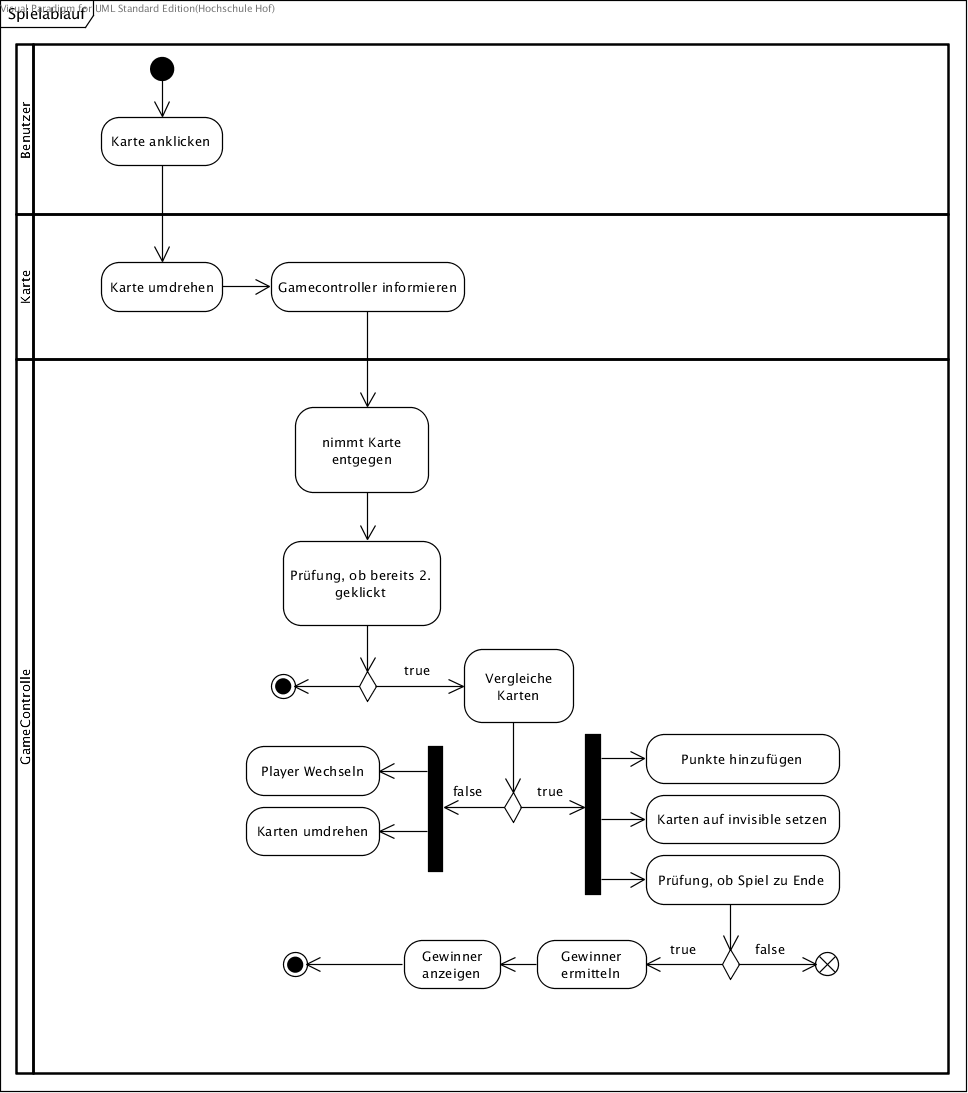
\includegraphics[width=\textwidth]{./AD_Spielablauf.png}
	\label{layout_gesamt}
\end{figure}
\subsection{Beschreibung}
Der Spielablauf beginnt mit dem Klick auf eine Karte durch den Benutzer. In der Klasse Card (Karte) wird die Funktion zum Umdrehen der Karte aufgerufen und der GameController wird informiert, dass eine Karte ausgewählt wurde. Der GameController nimmt die Information über die Karte entgegen und prüft, ob es sich um die 2. ausgewählte Karte handelt. Ergibt diese Prüfung false, ist die Aktivität beendet. Erst durch den nächsten Klick auf eine Karte, wird die Aktivität wiederholt. Hat die Prüfung true ergeben, erfolgt ein Vergleich der durch den Benutzer gewählten Karten. False führt dazu, dass der Spieler gewechselt wird, die Karten wieder umgedreht werden und die Aktivität beendet ist. Bei True werden dem aktuellen Spieler Punkte hinzugefügt, die Karten auf invisible gesetzt und eine Prüfung angestoßen, ob das Spielende erreicht ist. Ist das Spielende nicht erreicht, endet die Aktivität. Ergibt die Prüfung, dass das Spielende erreicht ist, wird der Gewinner ermittelt und angezeigt. Hier endet die Aktivität.


\clearpage
\section{Komponentendiagramm}

\begin{figure}[!h]
	\centering
    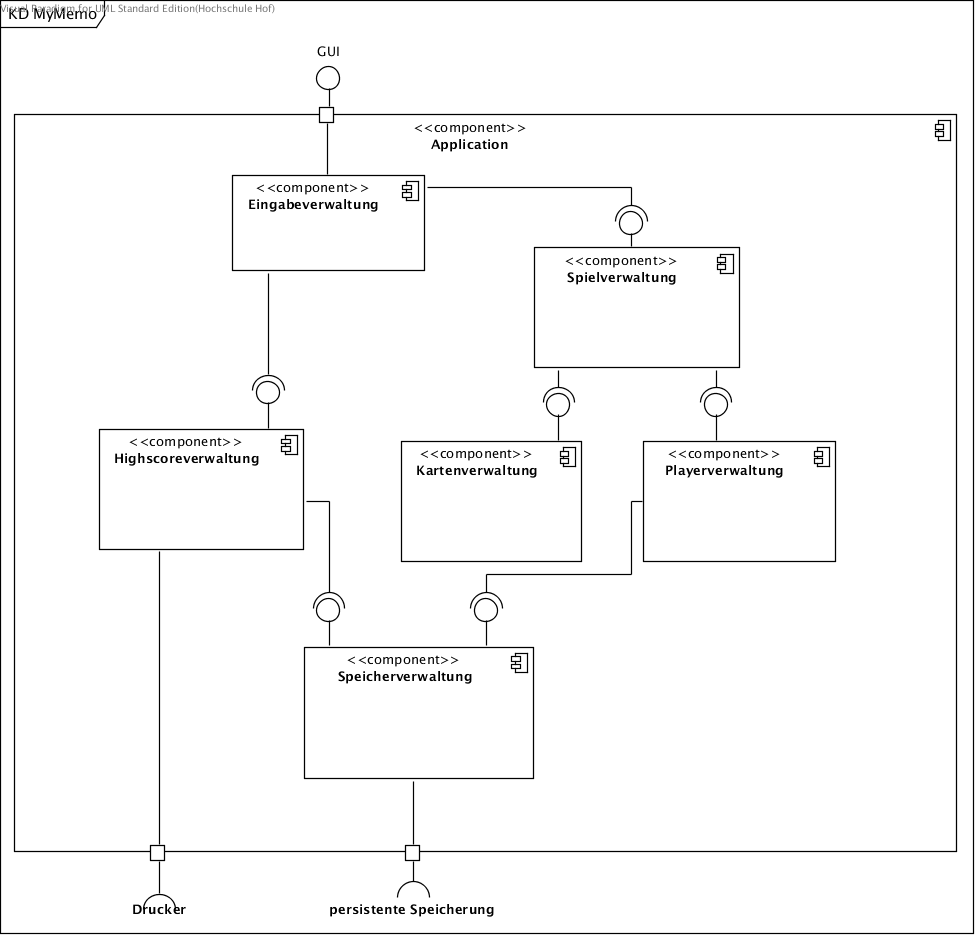
\includegraphics[width=\textwidth]{./komponentendiagramm.png}
	\label{layout_gesamt}
\end{figure}
\subsection{Beschreibung}
Um eine bessere Übersicht zu erhalten, wurden die Klassen aus dem Klassendiagramm zu Komponenten zusammengefasst.\\

\noindent \textbf{Eingabeverwaltung: }Menue, InputData\\
\textbf{Spielverwaltung: }GameField, GameLayout, GameController\\
\textbf{Playerverwaltung: }Player, Playerpool\\
\textbf{Kartenverwaltung: }Card\\
\textbf{Highscoreverwaltung: }Highscore, HighscoreData\\
\textbf{Speicherverwaltung: }SaveObject, HddSave\\

Das Komponentendiagramm stellt dar, wie die einzelnen Komponenten des Systems aufeinander zugreifen.\\
Die Applikation selbst hat Schnittstellen zur Technischen Schicht in Form von Drucker und persistenter Speicherung. Eine weitere Schnittstelle besteht zur Präsentationsschicht, im Diagramm zusammengefasst unter GUI.



\clearpage
\section{Paketdiagramm}

\begin{figure}[!h]
	\centering
    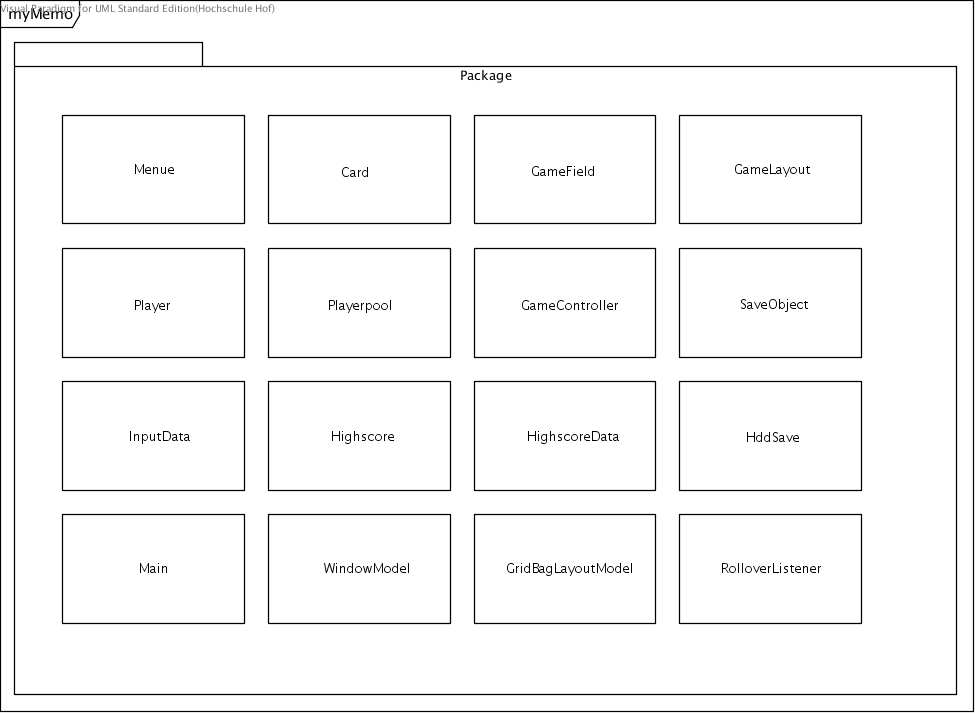
\includegraphics[width=\textwidth]{./paketdiagramm.png}
	\label{layout_gesamt}
\end{figure}
\subsection{Beschreibung}
Da das System ohne die Verwendung verschiedener Packages geplant und umgesetzt wurde, erfolgt die Darstellung des Paketdiagramms in obiger Form.


\clearpage
\section{Verteilungsdiagramm}

\begin{figure}[!h]
	\centering
    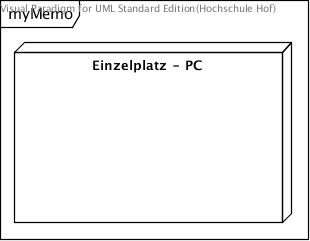
\includegraphics[width=\textwidth]{./verteilungsdiagramm.png}
	\label{layout_gesamt}
\end{figure}
\subsection{Beschreibung}
Die Software kommt ausschließlich auf Einzelplatz-PCs zum Einsatz. Es erfolgt keine Verteilung auf verschiedene Systeme. Deshalb enthält das Verteilungsdiagramm ausschließlich den Einzelplatz-PC.





\clearpage

\chapter{Implementierung}

\section{Allgemeines}
Die Implementierung wurde für alle Lastenheftfunktionen der Priorität 1 umgesetzt. Alle Elemente der grafischen Benutzeroberfläche sind ohne GUI-Builder erstellt worden. Der Programmcode liegt als .java Dateien vor und kann über den Aufruf von Main.java ausgeführt werden.

\section{Umfang}
Es wurden 16 Klassen mit insgesamt X Lines of Code implementiert.

\begin{figure}[!h]
	\centering
    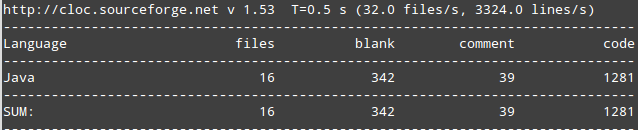
\includegraphics[width=\textwidth]{./cloc.png}
	\label{layout_gesamt}
\end{figure}


%GUI
\clearpage
\section{Benutzerobefläche}

\subsection{Hauptmenue}
\begin{figure}[!h]
	\centering
    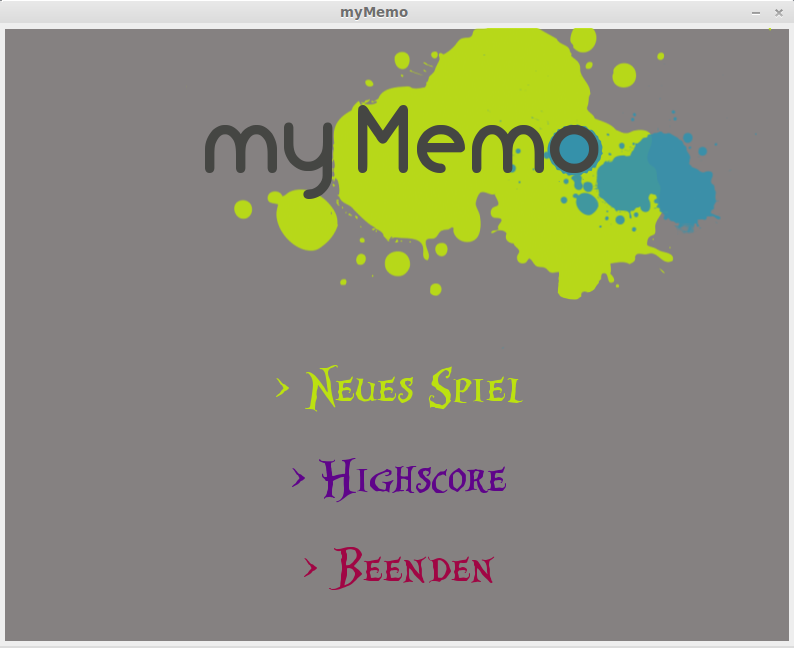
\includegraphics[width=\textwidth]{./guiHauptmenue.png}
	\label{}
\end{figure}
\paragraph{Beschreibung: } Im Hauptmenue kann der Benutzer zwischen den Optionen ,,Neues Spiel``, ,,Highscore`` und ,,Beenden`` wählen. Die Option ,,Neues Spiel`` öffnet Eingabemasken zur Erfassung des Namens und weiterer Wahlmöglichkeiten. Ein Click auf ,,Highscore`` zeigt die aktuelle Highscore an. Der Button Beenden schließt die Anwendung.  


\clearpage
\subsection{Neues Spiel - Spielmodus wählen}
\begin{figure}[!h]
	\centering
    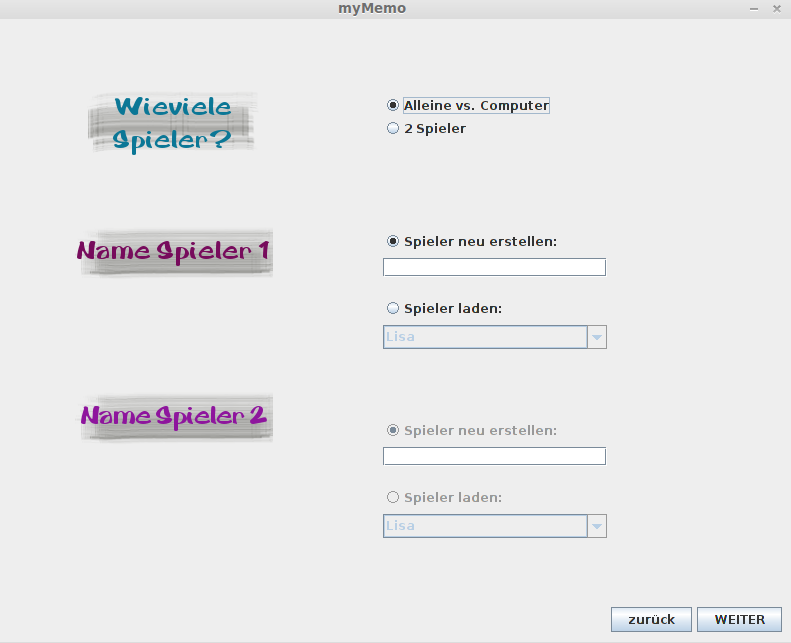
\includegraphics[width=\textwidth]{./guiSpieler.png}
	\label{}
\end{figure}
\paragraph{Beschreibung: }Wurde ,,Neues Spiel'' gewählt, erscheint die obige Maske. In diesem Fall wurde der Spielmodus ,,Alleine vs. Computer'' gewählt. Die Auswahl schaltet die Eingabefelder für den Namen von Spieler 1 frei. Die Eingabefelder von Spieler 2 werden nicht benötigt und sind deshalb nicht editierbar. Der Button ,,zurück'' würde den Benutzer zum Hauptmenue leiten, der Button ,,WEITER'' zur nächsten Eingabemaske für Thema und Spielfeldgröße.

\clearpage
\subsection{Neues Spiel - Spieler erstellen}
\begin{figure}[!h]
	\centering
    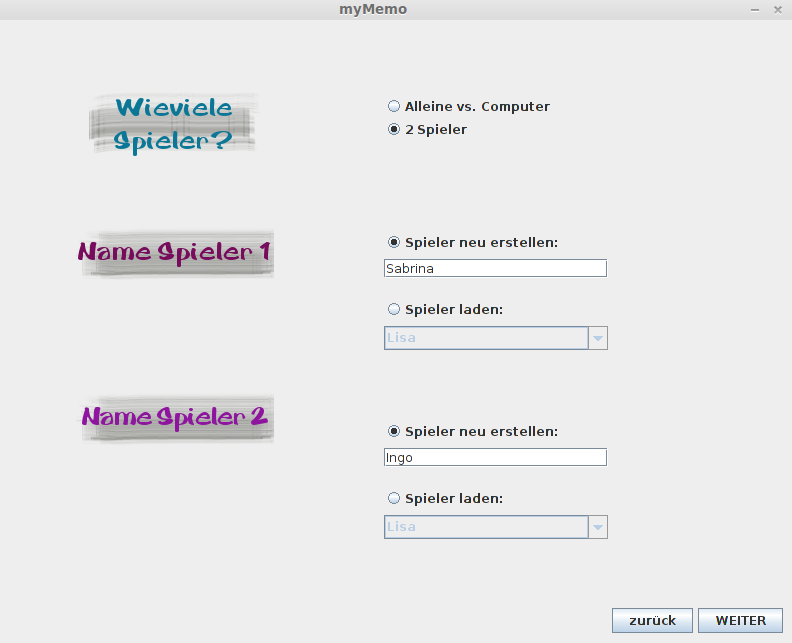
\includegraphics[width=\textwidth]{./guiSpielerNeu.png}
	\label{}
\end{figure}
\paragraph{Beschreibung: }Es wurde der 2-Spieler-Modus gewählt. Nun sind die Eingabefelder für Name von Spieler 1 und Spieler 2 aktiv. Hier wurde in beiden Fällen ein neuer Name erfasst.


\clearpage
\subsection{Neues Spiel - Spieler aus Liste wählen}
\begin{figure}[!h]
	\centering
    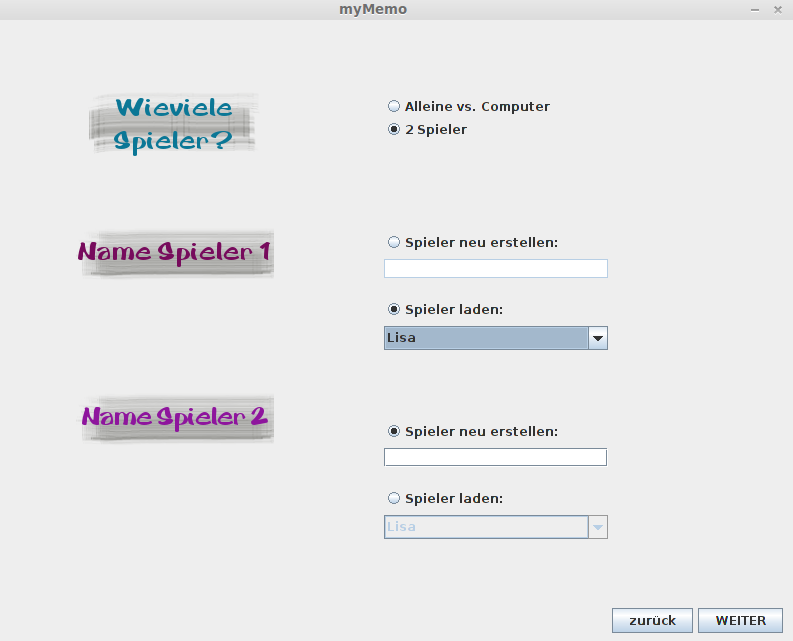
\includegraphics[width=\textwidth]{./guiSpielerListe.png}
	\label{}
\end{figure}
\paragraph{Beschreibung: }Durch den Klick auf den Radiobutton ,,Spieler laden'' wird eine Liste als Dropdown-Menue bereitgestellt. Aus dieser können gespeicherte Namen gewählt werden.


\clearpage
\subsection{Neues Spiel - Prüfung auf doppelten Namen}
\begin{figure}[!h]
	\centering
    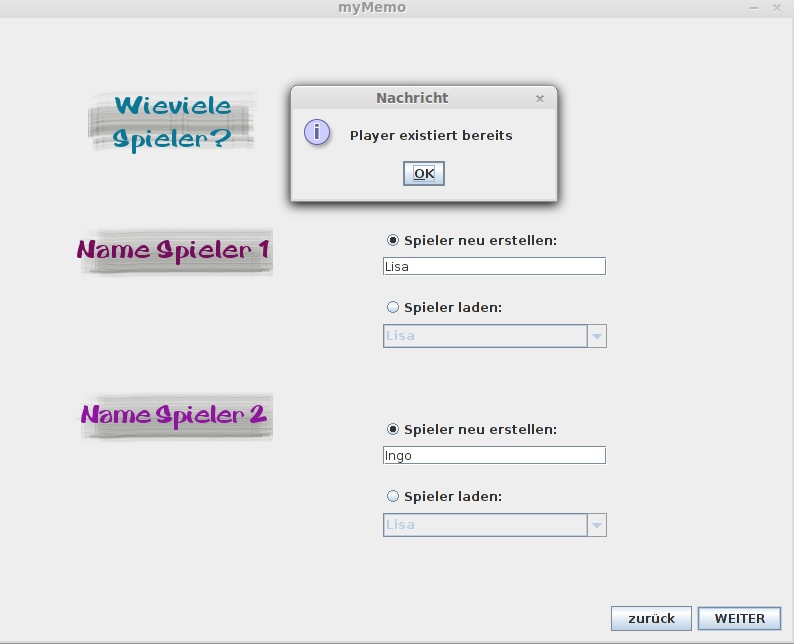
\includegraphics[width=\textwidth]{./guiSpielerError.png}
	\label{}
\end{figure}
\paragraph{Beschreibung: }Bei der Eingabe eines Namens zur Erstellung eines neuen Spielers prüft das System, ob der Name bereits existiert und gibt eine Fehlermeldung aus. Erst nach Änderung und erneuter Prüfung wird durch den Klick auf ,,WEITER'' die nächste Maske aufgerufen.

\clearpage
\subsection{Neues Spiel - Thema und Spielfeldgröße}
\begin{figure}[!h]
	\centering
    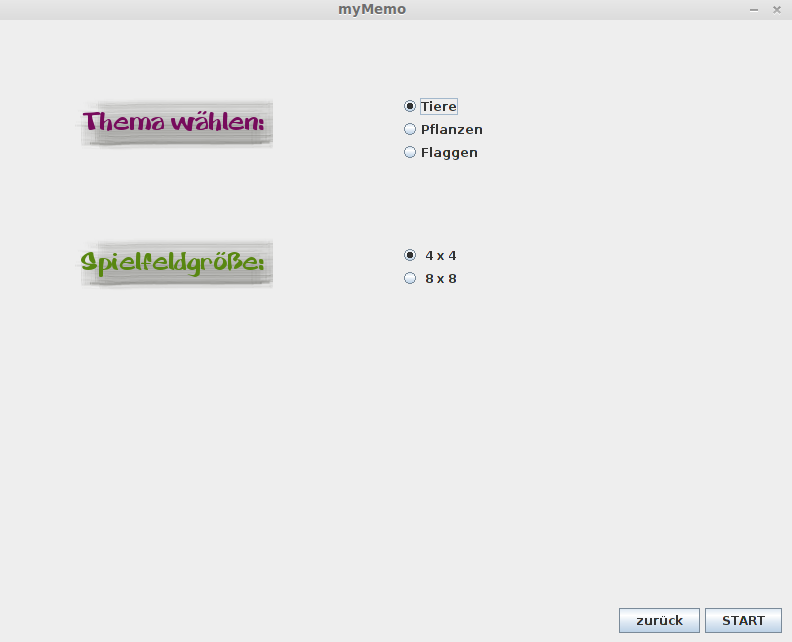
\includegraphics[width=\textwidth]{./guiTiere.png}
	\label{}
\end{figure}
\paragraph{Beschreibung: }Nach Wahl des Spielmodus und Eingabe oder Auswahl des Namens erscheint obige Maske. Hier kann zwischen den Karenthemen Tiere, Pflanzen und Flaggen gewählt werden. Bei der Spielfeldgröße gibt es die Option 4x4 oder 8x8 Karten. Der Kick auf den Button ,,START'' startet das Spiel.


\clearpage
\subsection{Spielfeld}
\begin{figure}[!h]
	\centering
    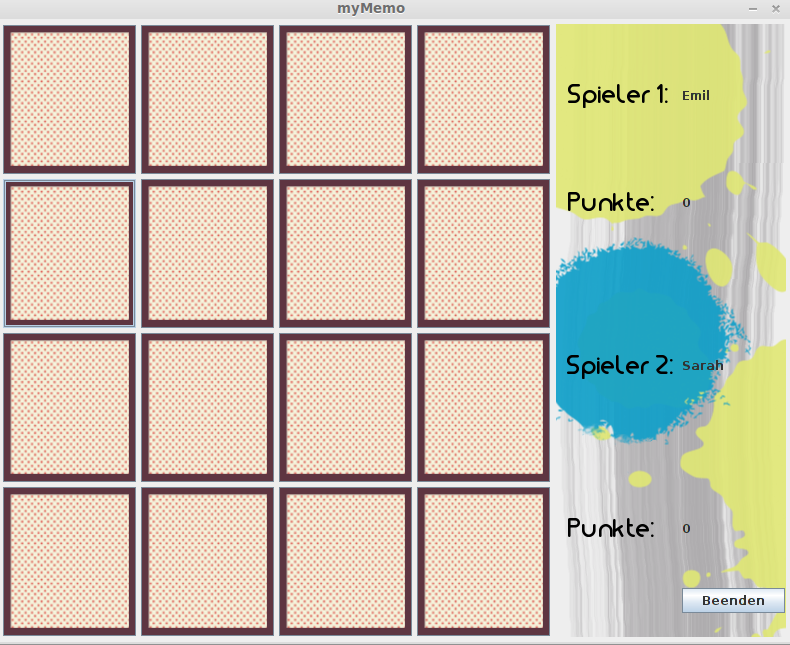
\includegraphics[width=\textwidth]{./guiSpielfeld.png}
	\label{}
\end{figure}
\paragraph{Beschreibung: }Links: Spielfeld mit gemischten Karten und ausgewählten Kartenmotiven. Rechts: Anzeige der Spielerdaten. Es werden die Namen der Spieler und die aktuellen Punkte angezeigt.


\clearpage
\subsection{Spielfeld - Karten gewählt}
\begin{figure}[!h]
	\centering
    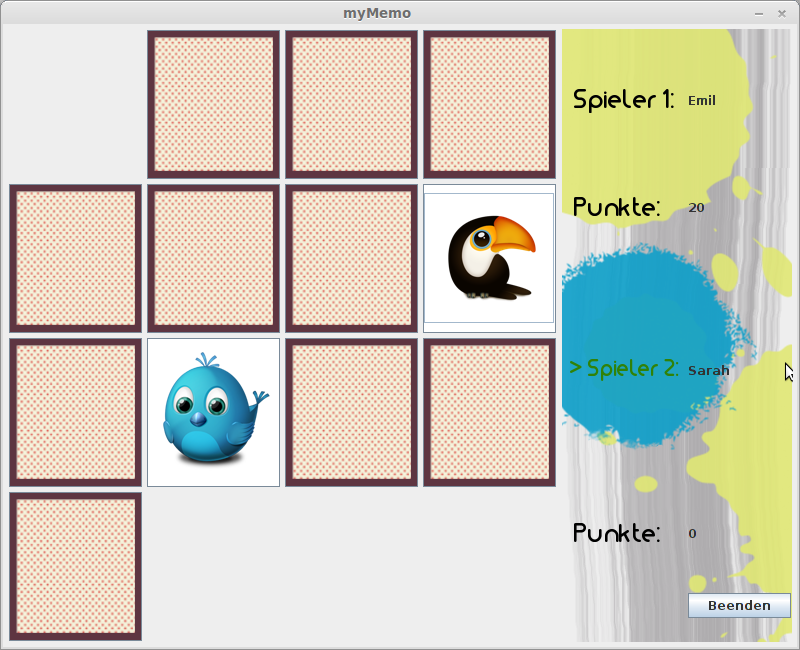
\includegraphics[width=\textwidth]{./guiSpielCards.png}
	\label{}
\end{figure}
\paragraph{Beschreibung: }In dieser Spielsituation hat der Spieler Emil bereits zwei übereinstimmende Kartenpaare gewonnen und somit 20 Punkte erspielt. Jetzt ist Sarah an der Reihe, was durch die farbige Markierung von ,,Spieler 2'' zu erkennen ist. Es sind zwei Karten vom Kartenthema Tiere aufgedeckt.


\clearpage
\subsection{Spielende - Anzeige Gewinnner}
\begin{figure}[!h]
	\centering
    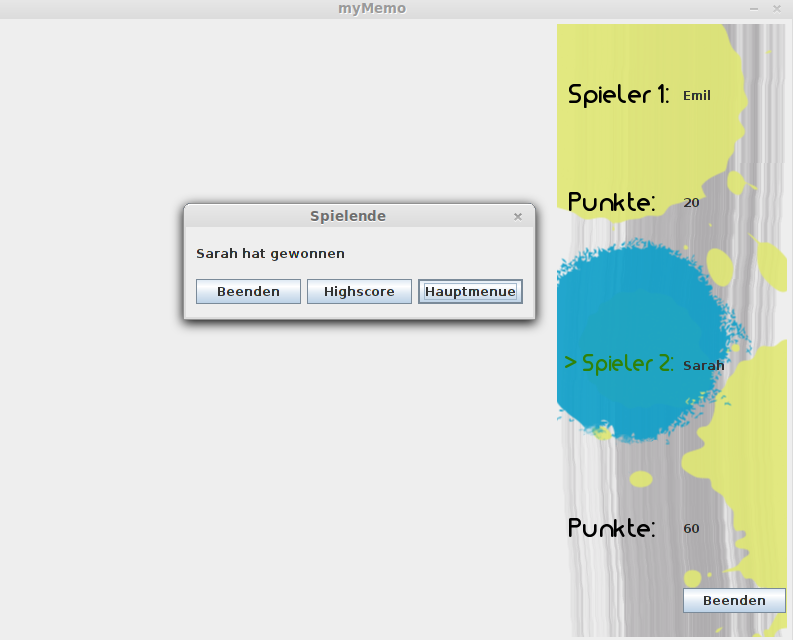
\includegraphics[width=\textwidth]{./guiSpielende.png}
	\label{}
\end{figure}
\paragraph{Beschreibung: }Am Ende des Spiels d.h. wenn alle übereinstimmenden Kartenpaare gefunden wurden, erscheint ein Meldedialog, der den Gewinner mitteilt. Hier hat Sarah mit 60 Punkten gewonnen.


\clearpage
\subsection{Highscore anzeigen}
\begin{figure}[!h]
	\centering
    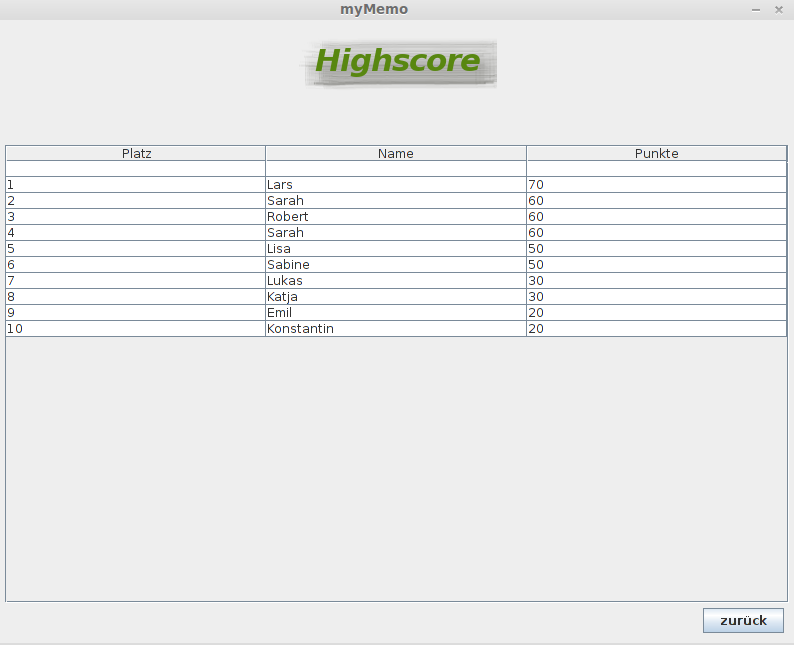
\includegraphics[width=\textwidth]{./guiHighscore.png}
	\label{}
\end{figure}
\paragraph{Beschreibung: } Anzeige der Highscore. Die 10 besten Spieler werden mit ihren erreichten Punkten in Form einer Tabelle aufgelistet.


\clearpage

\chapter{Test}

\section{Testfall 1 - Spielmodus: Gegen Computer}
\begin{figure}[!h]
	\centering
    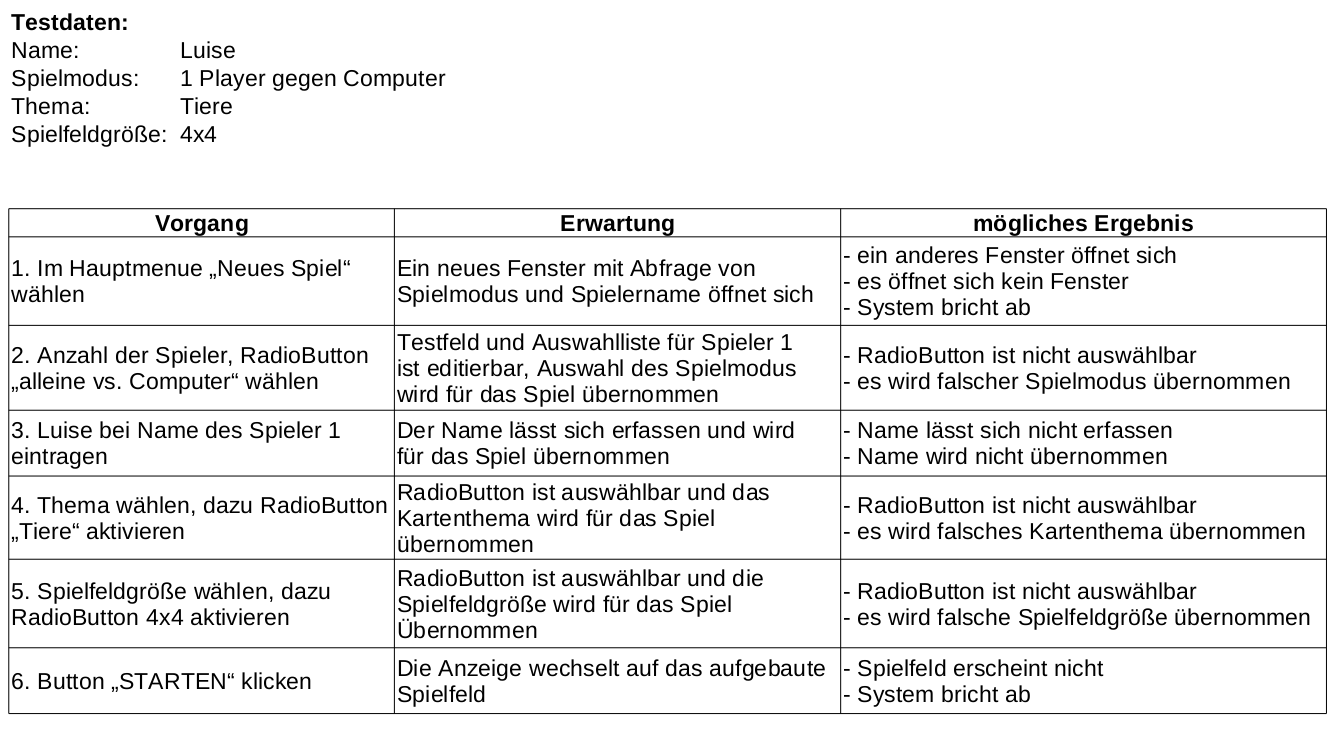
\includegraphics[width=15cm]{./Testfall1.png}
	\label{layout_gesamt}
\end{figure}

\end{document}
